
\title{A Comparison of Dimensionality Reduction Techniques for Robotic Motion
Planning}

\date{\today}

\author{Brandon Araki \and Alex Wallar}

\documentclass[12pt]{article}

\usepackage[pdftex]{graphicx}
\graphicspath{ {figs/} }
\usepackage{subcaption}

\usepackage{amsmath}
\usepackage{amssymb}
\usepackage{mathabx}

\usepackage{relsize}

\usepackage{float}

\usepackage{algorithm}

\usepackage[noend]{algorithmic}

\floatstyle{ruled} \newfloat{program}{thp}{lop} \floatname{program}{Structure}

\newcommand{\Normal}[3]{\mathcal{N}(#1, #2, #3)}

\newcommand{\Acronym}[1]{\ensuremath{{\small{\texttt{#1}}}}}
\newcommand{\Name}{\Acronym{Camgaze.js}} \newcommand{\False}{\Constant{false}}
\newcommand{\True}{\Constant{true}}
\newcommand{\Symbol}[1]{\ensuremath{\mathcal{#1}}}
\newcommand{\Function}[1]{\ensuremath{{\small \textsc{#1}}}}
\newcommand{\Constant}[1]{\ensuremath{\small{\texttt{#1}}}}
\newcommand{\Var}[1]{\ensuremath{{\small{\textsl{#1}}}}}
\newcommand{\argmin}[1]{\underset{#1}{\operatorname{arg}\,\operatorname{min}}\;}
\newcommand{\grad}[1]{\underset{#1}{\operatorname{\Function{GradientDecent}}}\;}

\newcommand{\xr}[0]{\ensuremath{{x_{\Var{rand}}}}}
\newcommand{\xnear}[0]{\ensuremath{{x_{\Var{near}}}}}
\newcommand{\xnearest}[0]{\ensuremath{{x_{\Var{nearest}}}}}
\newcommand{\xnew}[0]{\ensuremath{{x_{\Var{new}}}}}
\newcommand{\xmin}[0]{\ensuremath{{x_{\Var{min}}}}}
\newcommand{\xparent}[0]{\ensuremath{{x_{\Var{parent}}}}}
\newcommand{\cmin}[0]{\ensuremath{{c_{\Var{min}}}}}
\newcommand{\cost}[0]{\ensuremath{{\Function{Cost}}}}
\newcommand{\linef}[1]{\ensuremath{{c(\Function{Line}(#1))}}}

\begin{document}

\maketitle

\section{Background}

Dimensionality reduction is a key component of making robotic motion planning
fast and efficient. A rigid body has six degrees of freedom (DoF), so a
multi-link robot such as a humanoid or snake robot can have dozens or hundreds
of DoF. The rotational and translational transformations of a rigid body can be
described with the 3-dimensional Special Euclidean group (known as SE(3)).
SE(3) is homeomorphic to the topological space $\mathbb{R}^3\bigtimes\mathbb{RP}^3$ (where $\mathbb{RP}^3$ is the
3-dimensional real projective plane). Therefore it is easy to imagine a
multi-link robot \cite{kuindersma2015optimization} or a multi-robot system \cite{alonso2015multi} with an arbitrarily complex state space. The picture is
further complicated by the addition of obstacles into a robot's world. The
state space for motion planning, which must take into account both the robot
and obstacles, is called the configuration space (or C-space) \cite{lozano1983spatial}. 

Motion planning essentially consists of a search over the configuration space
from a start configuration to a goal configuration. A huge number of methods
for searching through the configuration space have been developed, most of
which can be divided into two classes, sampling-based motion planning and
combinatorial motion planning \cite{lavalle2006planning}. In sampling-based motion planning, obstacles in
the C-space are defined implicitly so that the path is constructed by randomly
or pseudorandomly sampling points from the C-space and doing collision
checking. In combinatorial motion planning, obstacles are defined explicitly
and a complete search of the C-space is made. Because of the difficulty of
explicitly defining all of the geometry in a potentially complex world,
sampling-based motion planning techniques such as the Rapidly-exploring Random
Tree (RRT) and Probabilistic RoadMap (PRM) planning are the most popular motion
planning techniques.

We used RRT* and PRM* in our project. The * indicates that these are the
asymptotically optimal versions of RRT and PRM (they are guaranteed to find the
optimal path as time goes to infinity).

The Probabilistic RoadMap algorithm has two phases: the preprocessing phase in which a roadmap is constructed by sampling random points in the C-space, and the query phase in which a graph search over the roadmap is made to connect initial and goal configurations \cite{kavraki1996prm}. The map is constructed during the preprocessing phase by sampling random points in the C-space and then adding them to the vertices in the roadmap within a certain radius of the point. PRM can be elevated to the asymptotically optimal PRM*, which is described in Alg~\ref{alg:PRMstar}, by defining the radius to be a function of the number of vertices and the dimensionality of the space \cite{karaman2011sampling}.

The Rapidly exploring Random Tree algorithm works by building up a tree from the initial configuration to the goal configuration \cite{lavalle1998rrt}. Starting at the initial configuration of the root, it incrementally attempts to add randomly selected samples to the tree until it reaches the goal configuration. RRT*, which is described in Alg~\ref{alg:RRTstar} differs from RRT in that for every new node, connections are tested to the new node from every other node that is within a certain radius from the new node \cite{karaman2011sampling}. The the tree is pruned so that edges that are not part of the shortest path from the root of the tree to the new node are removed. 

\section{Problem Description}

Despite the efficiency of sampling-based search, the high dimensionality of the
configuration space of complex robots means that motion planning for many
robots is slow or infeasible. This is because of the ``curse of dimensionality",
in which the size of the search space increases exponentially with the
dimension. One way to speed up motion planning is to reduce the dimensionality
of the C-space and do search in this reduced dimensionality space. For this
project, we tested the performance of a number of dimensionality reduction
techniques to see which one was the most effective in speeding up motion
planning while providing reliable obstacle avoidance.

\section{Dimensionality Reduction}

We used Feature Agglomeration, Truncated SVD, PCA, Randomized PCA, and
our own ``Trained Johnson-Lindenstrauss" to perform dimensionality reduction. We will briefly summarize each of these techniques.

\textbf{PCA}: Principle Component Analysis, or PCA, transforms a set of variables into 
their ``principle components", or linearly uncorrelated variables. In other words, the axes of the dataset in question are reoriented so the Rayleigh quotient, which is related to the covariance of the dataset, along the first axis is maximized. After the first axis has been set, the second axis is then set to maximize the Rayleigh quotient of the dataset along that axis, and so on, so that the first axis has the highest Rayleigh quotient, the second axis has the second highest, and so on. Dimensionality reduction is then performed by chopping off the axes with the lowest Rayleigh quotients (which corresponded to axes with the lowest variance).

$$
\mathbf{w}_{(1)} = {\operatorname{\arg\,max}}\, \left\{ \frac{\mathbf{w}^T\mathbf{X}^T \mathbf{X w}}{\mathbf{w}^T \mathbf{w}} \right\}
$$

%Kernel PCA: Kernel PCA enables non-linear dimensionality reduction by using kernels to create a non-linear mapping from a high dimension to a lower dimension.

\textbf{Randomized PCA}: In Randomized PCA, computations are sped up by only approximating the singular vectors of the components.

\textbf{Feature Agglomeration}: Feature Agglomeration groups together similar features to reduce the number of features. It does this by using agglomerative clustering, in which every data point starts as a cluster, and clusters are merged together.

\textbf{Truncated SVD}: Truncated SVD works best with sparse matrices.

\textbf{Trained Johnson-Lindenstrauss}: Normal Johnson-Lindenstrauss uses a random mxn Gaussian matrix to reduce the dimensionality of a vector from n to m. Instead of using a random matrix, we train a matrix on randomly-generated obstacles in n-space to minimize [MINIMIZE WHAT?]

\section{Methods}

Simplifications: Although our aim is to show how dimensionality reduction techniques can speed up motion planning for robots, doing motion planning for an actual robot is extremely hard (specifying link geometry, defining constraints between links, etc). Therefore we limited ourselves to path planning for a point in $\mathbb{R}^n$, and we approximate obstacles as being convex polytopes. This is a valid simplification of the robot motion planning problem for several reasons. The first reason is that most real robots actually operate in a C-space similar to $\mathbb{R}^n$. This is because $\mathbb{RP}^3$, the space in which the rotation of a rigid body occurs, simplifies to $\mathbb{R}^3$ if the joint cannot make a full rotation. Second, in defining the C-space, the obstacle space takes into account the interaction of the robot geometry with obstacles. Therefore motion planning through the free space can be done using a point to represent the robot (since the geometry of the robot is implicitly included in the obstacle space). Therefore, although our simulations do not represent real robots and real obstacles, they do approximate them.

We implemented an n-dimensional world in which to test these algorithms. We structured our code so that we could run our tests in any space of dimension $d \geq 2$. We also made visualization scripts for the 2- and 3-dimensional tests (examples of which can be seen in Figs ~\ref{fig:2d_examples} and ~\ref{fig:3d_examples}).

Next we made a random obstacle generator. We create n-dimensional convex polytopes by sampling $n^{2}$ random points on the n-sphere using the equations below. 

\begin{align*}
x_1 &= r \cos(\phi_1) \\
x_2 &= r \sin(\phi_1) \cos(\phi_2) \\
x_3 &= r \sin(\phi_1) \sin(\phi_2) \cos(\phi_3) \\
    &\vdots\\
x_{n-1} &= r \sin(\phi_1) \cdots \sin(\phi_{n-2}) \cos(\phi_{n-1}) \\
x_n &= r \sin(\phi_1) \cdots \sin(\phi_{n-2}) \sin(\phi_{n-1}) \,.
\end{align*}

We then run Feature Agglomeration, Truncated SVD, PCA, Kernel PCA, and Randomized PCA to reduce the dimensionality of the space. We then run PRM* on each of these reduced dimensionality spaces, as well as on the full-dimensionality space as a control. We then run an inverse transform on the paths that we find to return them to the full-dimensionality space. Then we do collision checking and check the number of collisions the path makes with the obstacles.

\section{Results}

\begin{figure}[h!]
    \centering
    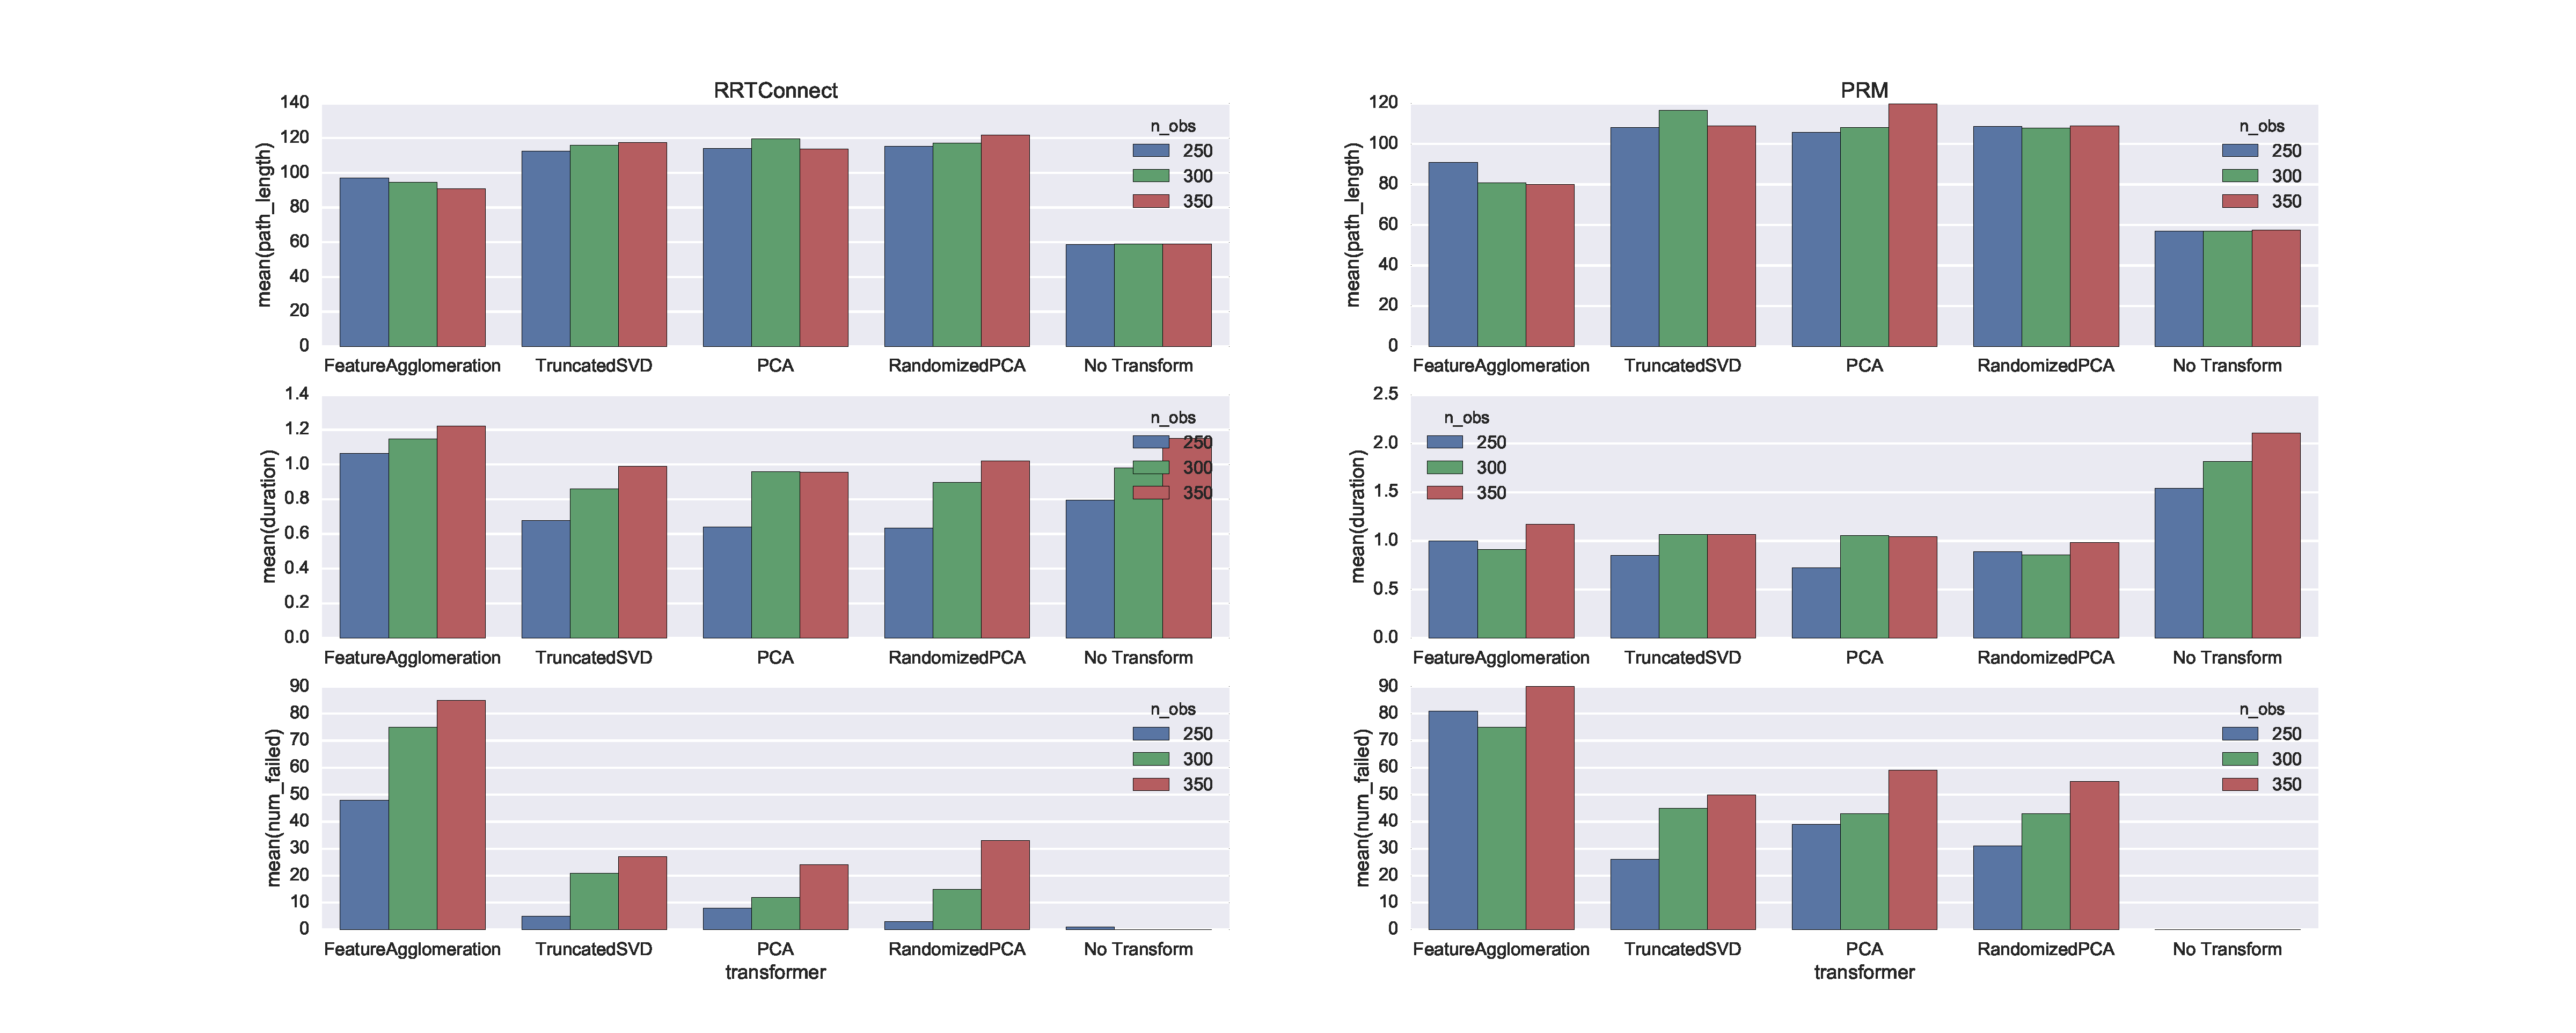
\includegraphics[width=\textwidth]{plots}
    \caption{Figure}
\end{figure}


\begin{figure}[t!]
    \centering
    \begin{subfigure}[t]{0.32\textwidth}
        \centering
        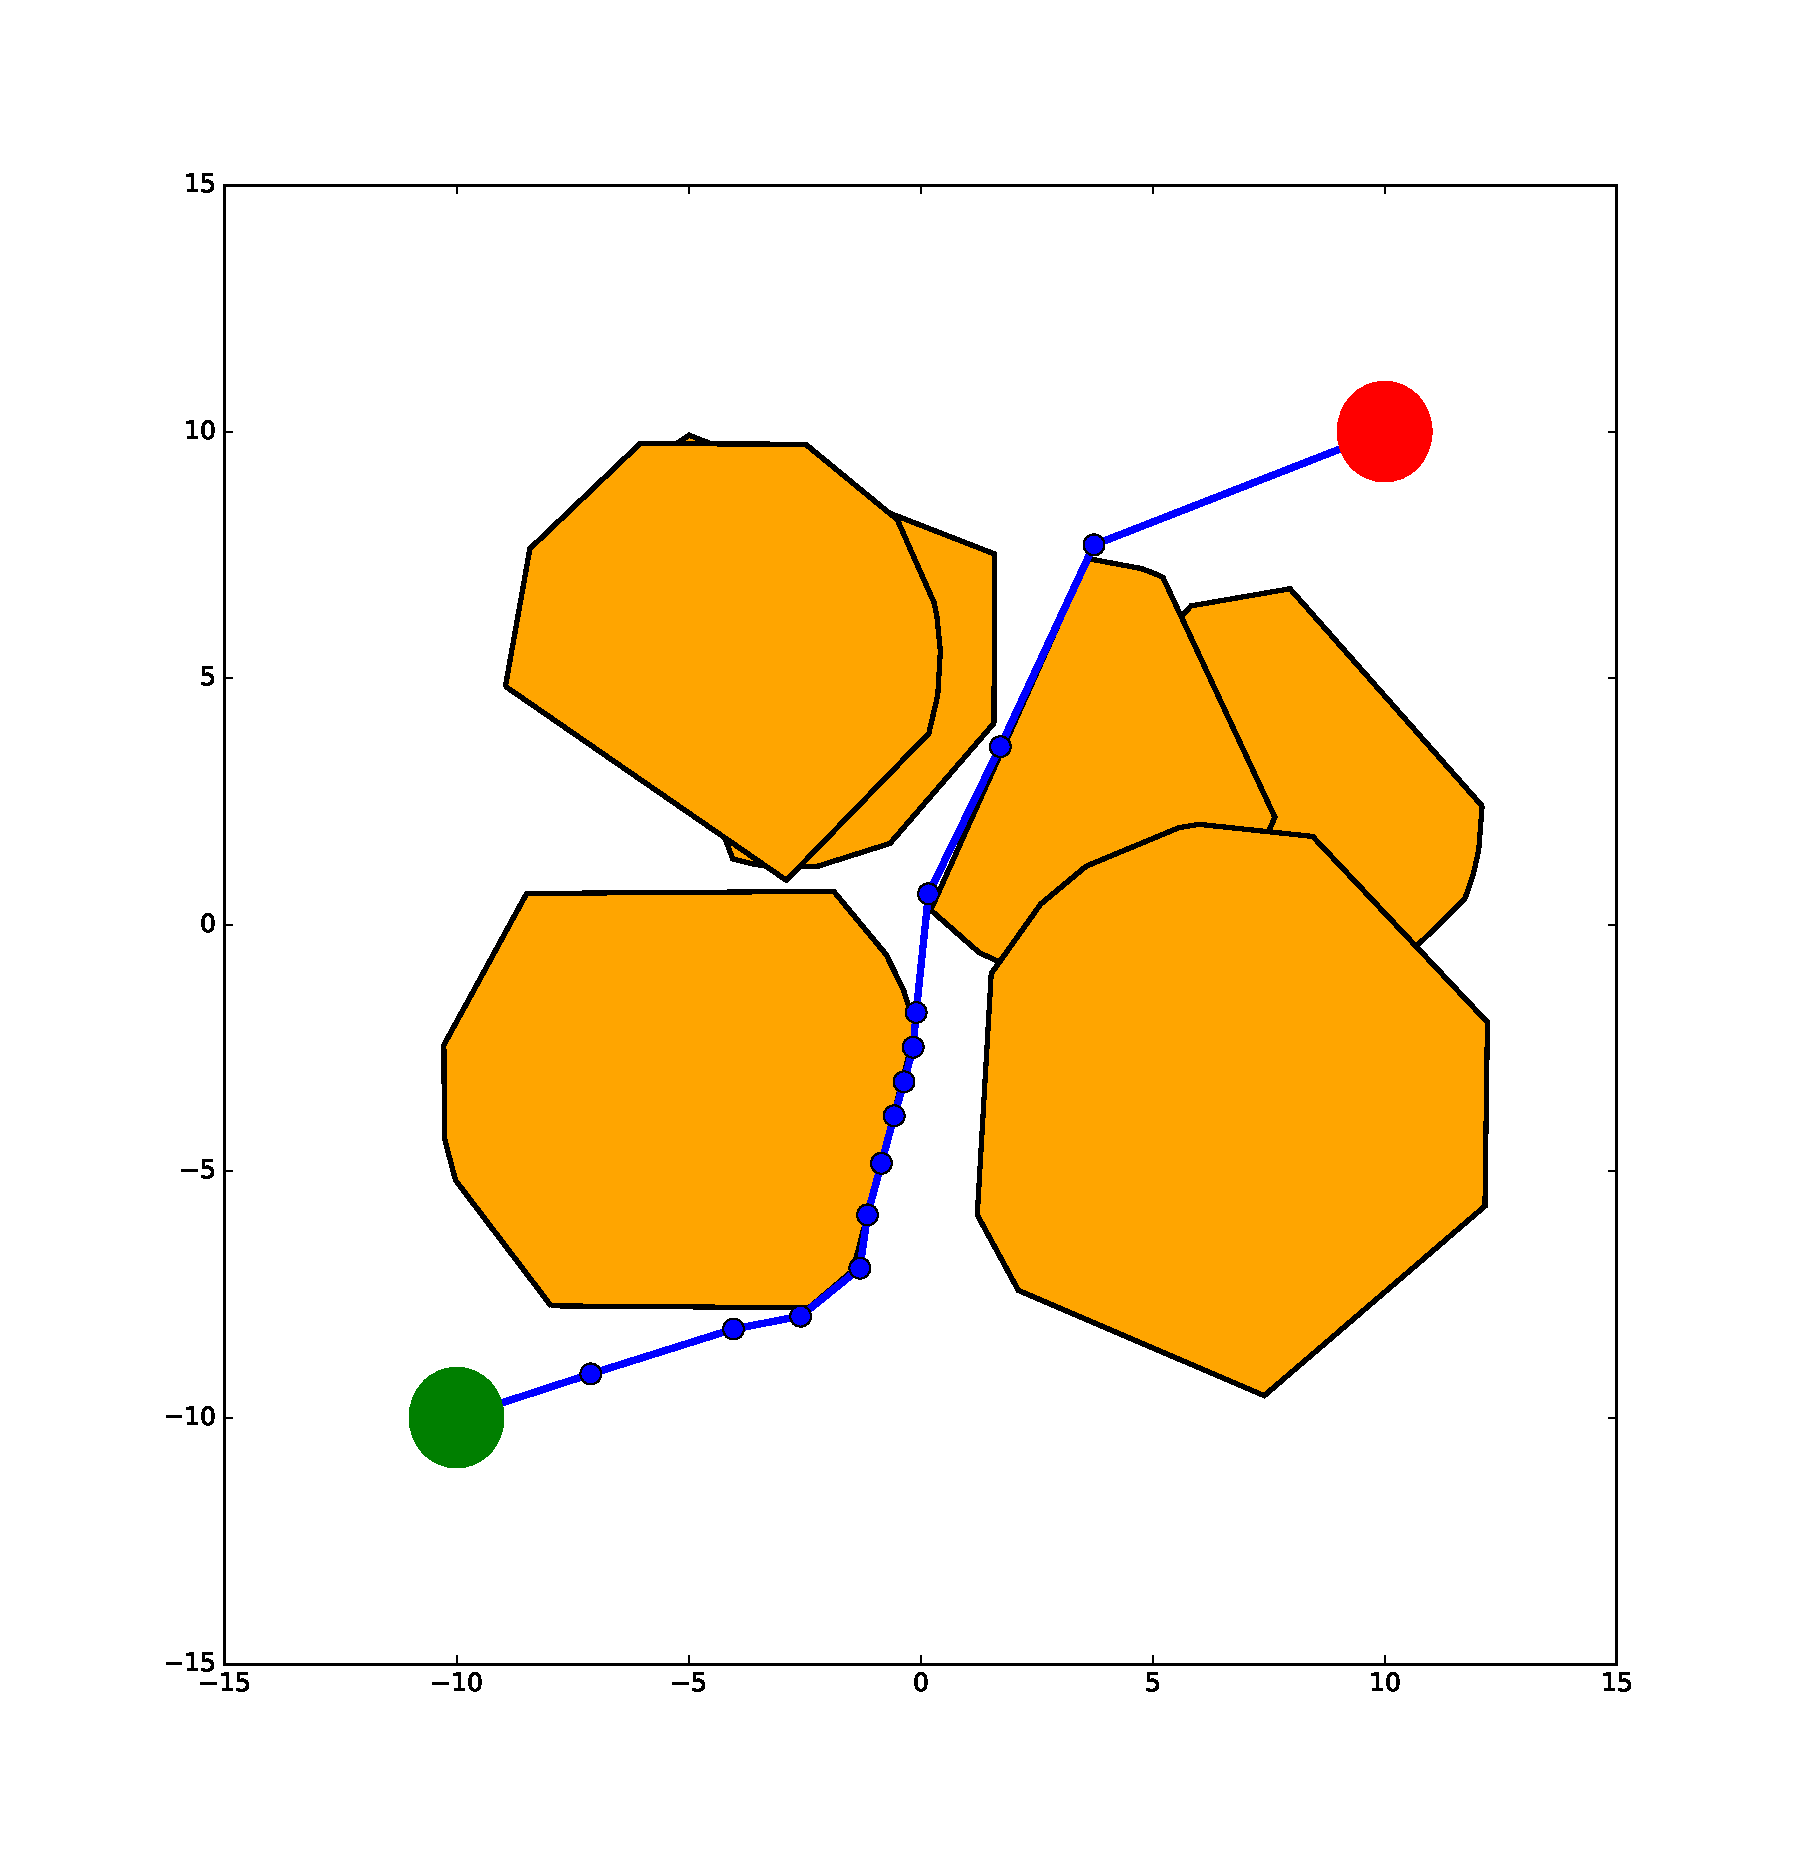
\includegraphics[width=\textwidth]{2d_example_1.pdf}
        \caption{a}
    \end{subfigure}%
    ~ 
    \begin{subfigure}[t]{0.32\textwidth}
        \centering
        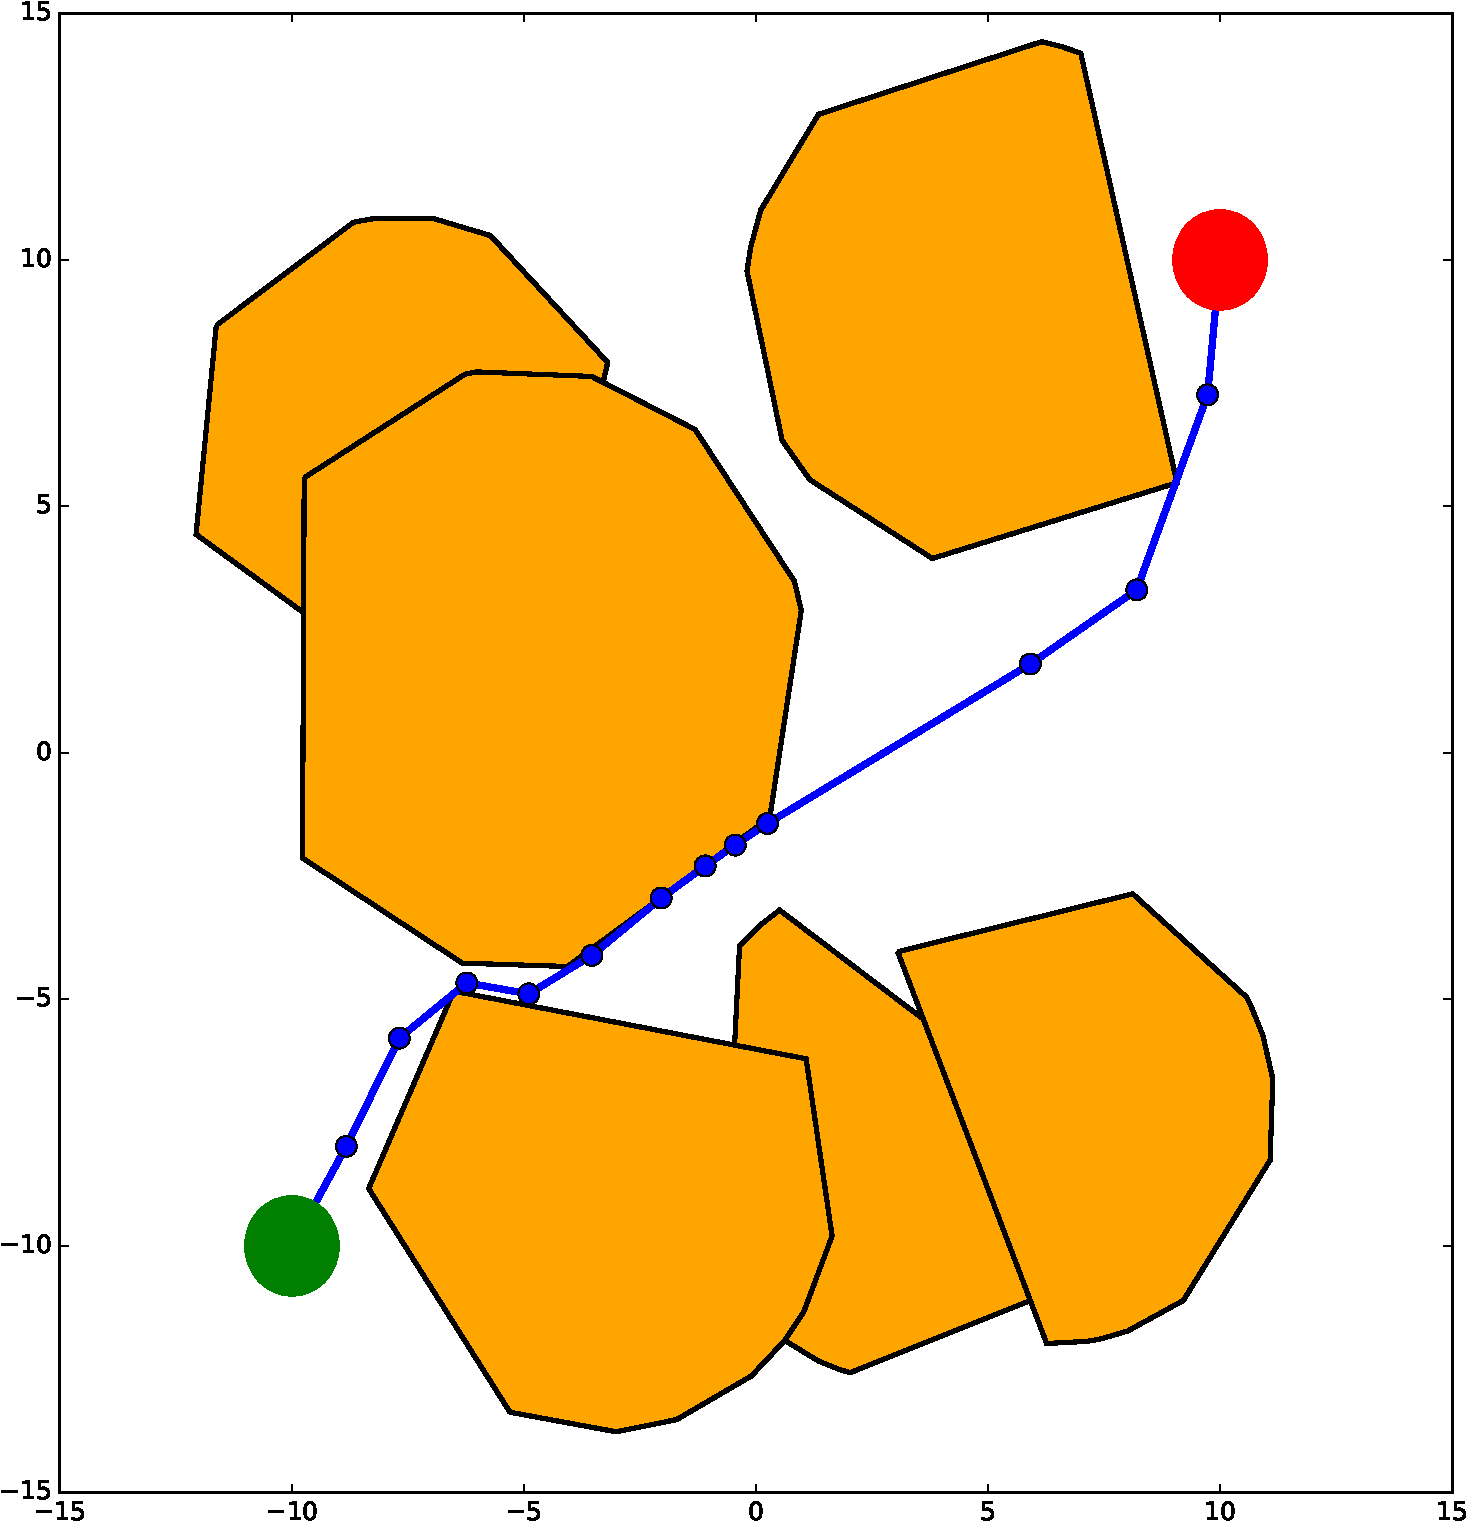
\includegraphics[width=\textwidth]{2d_example_2.pdf}
        \caption{b}
    \end{subfigure}
    \begin{subfigure}[t]{0.32\textwidth}
        \centering
        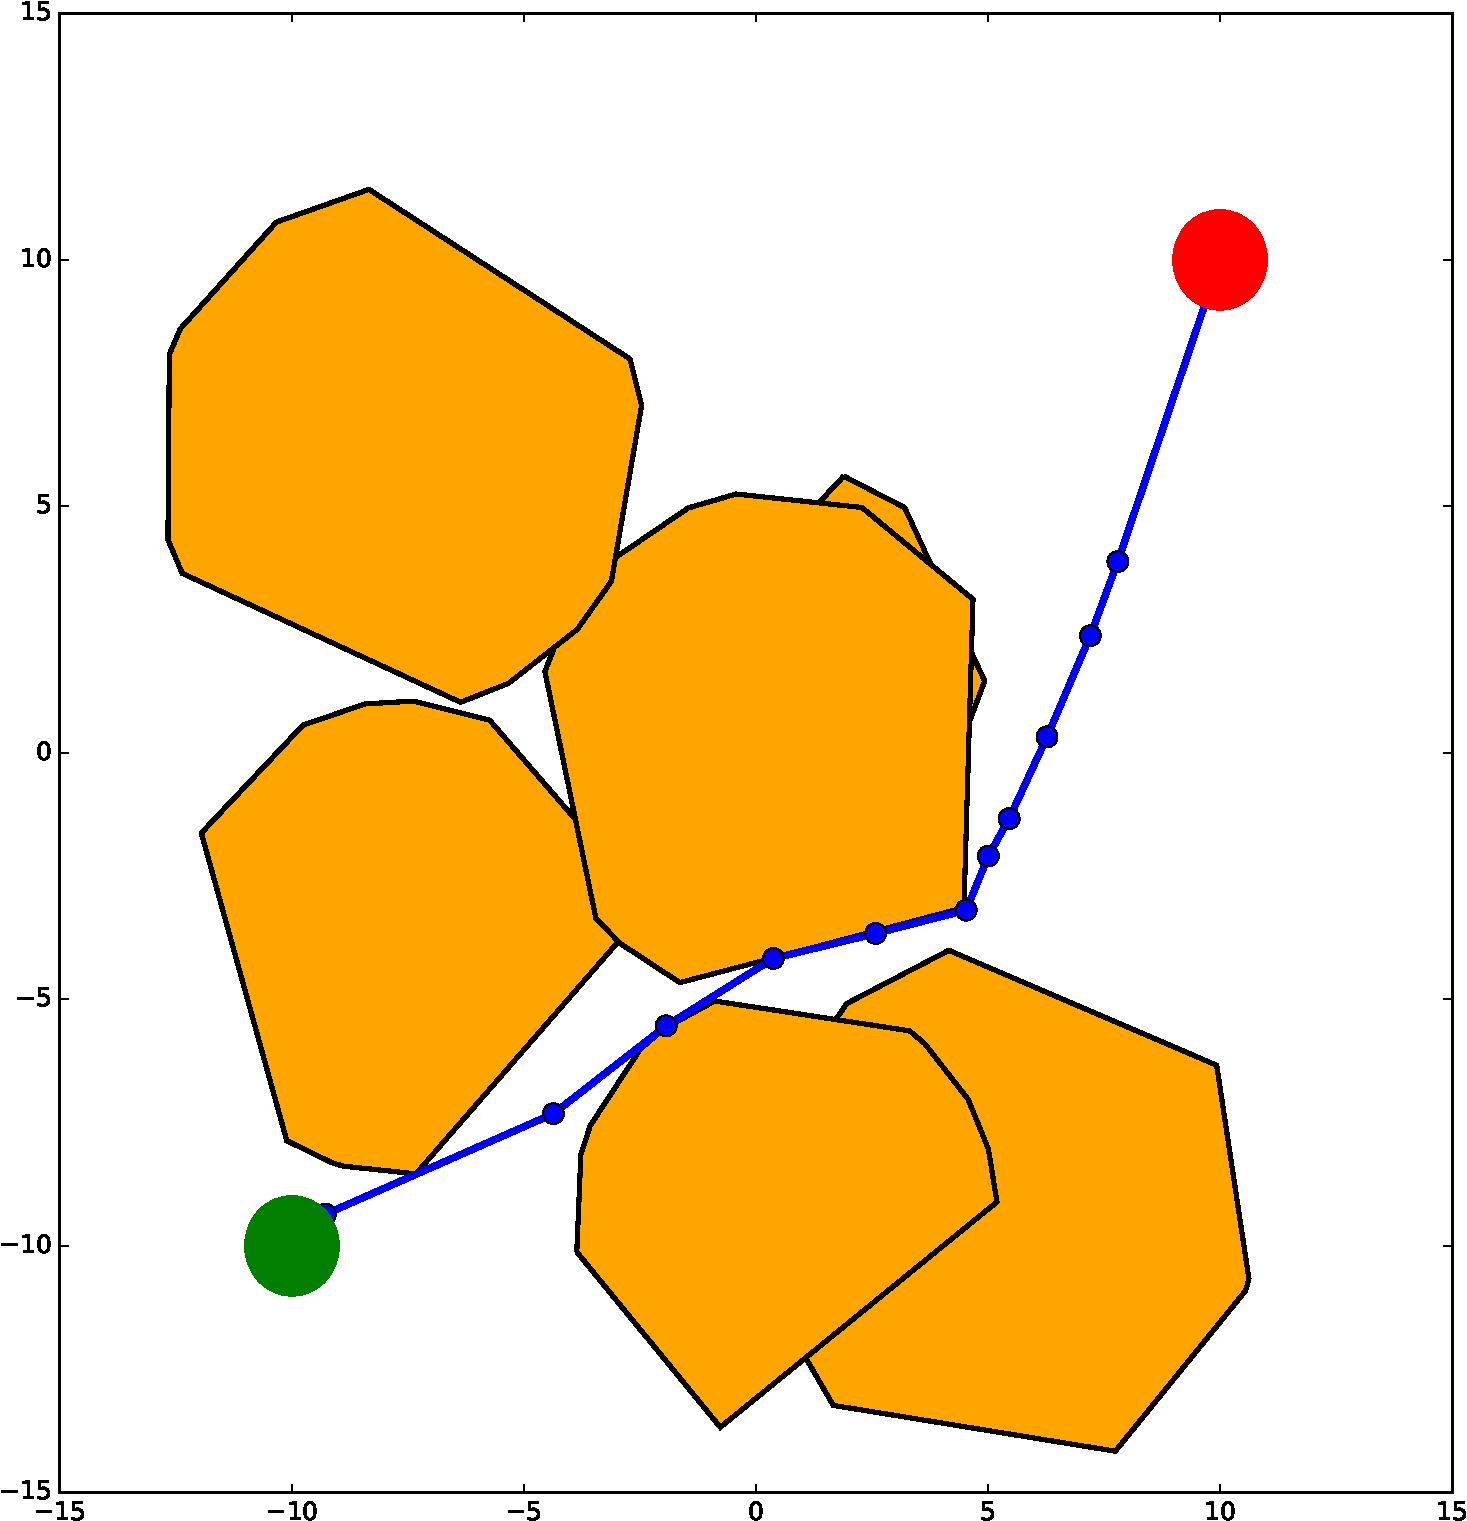
\includegraphics[width=\textwidth]{2d_example_3.pdf}
        \caption{c}
    \end{subfigure}
    \caption{2d examples}
    \label{fig:2d_examples}
\end{figure}

\begin{figure}[t!]
    \centering
    \begin{subfigure}[t]{0.32\textwidth}
        \centering
        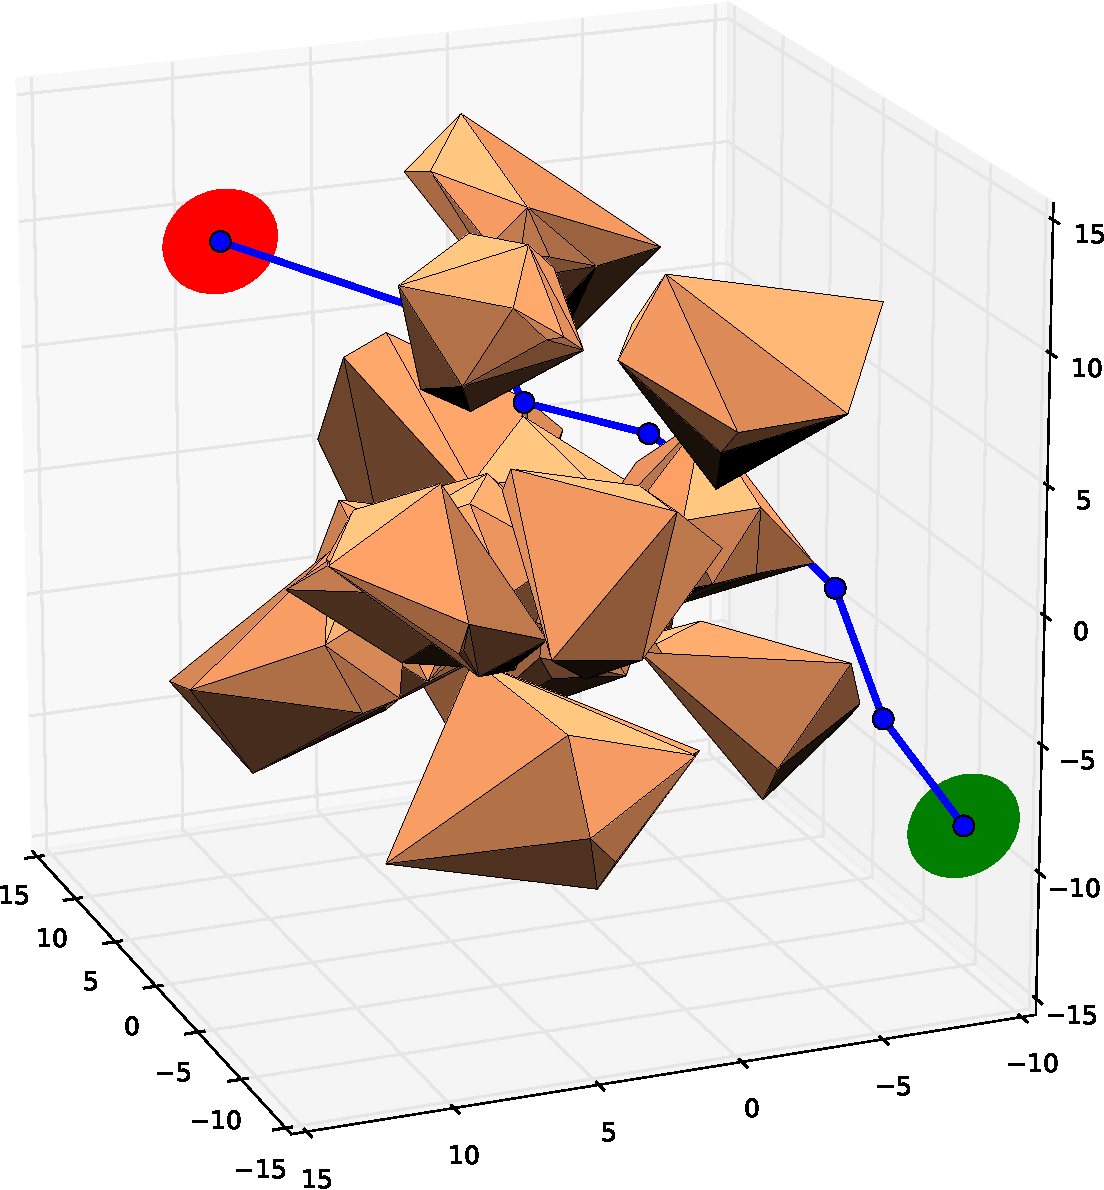
\includegraphics[width=\textwidth]{3d_example_1.pdf}
        \caption{a}
    \end{subfigure}%
    ~ 
    \begin{subfigure}[t]{0.32\textwidth}
        \centering
        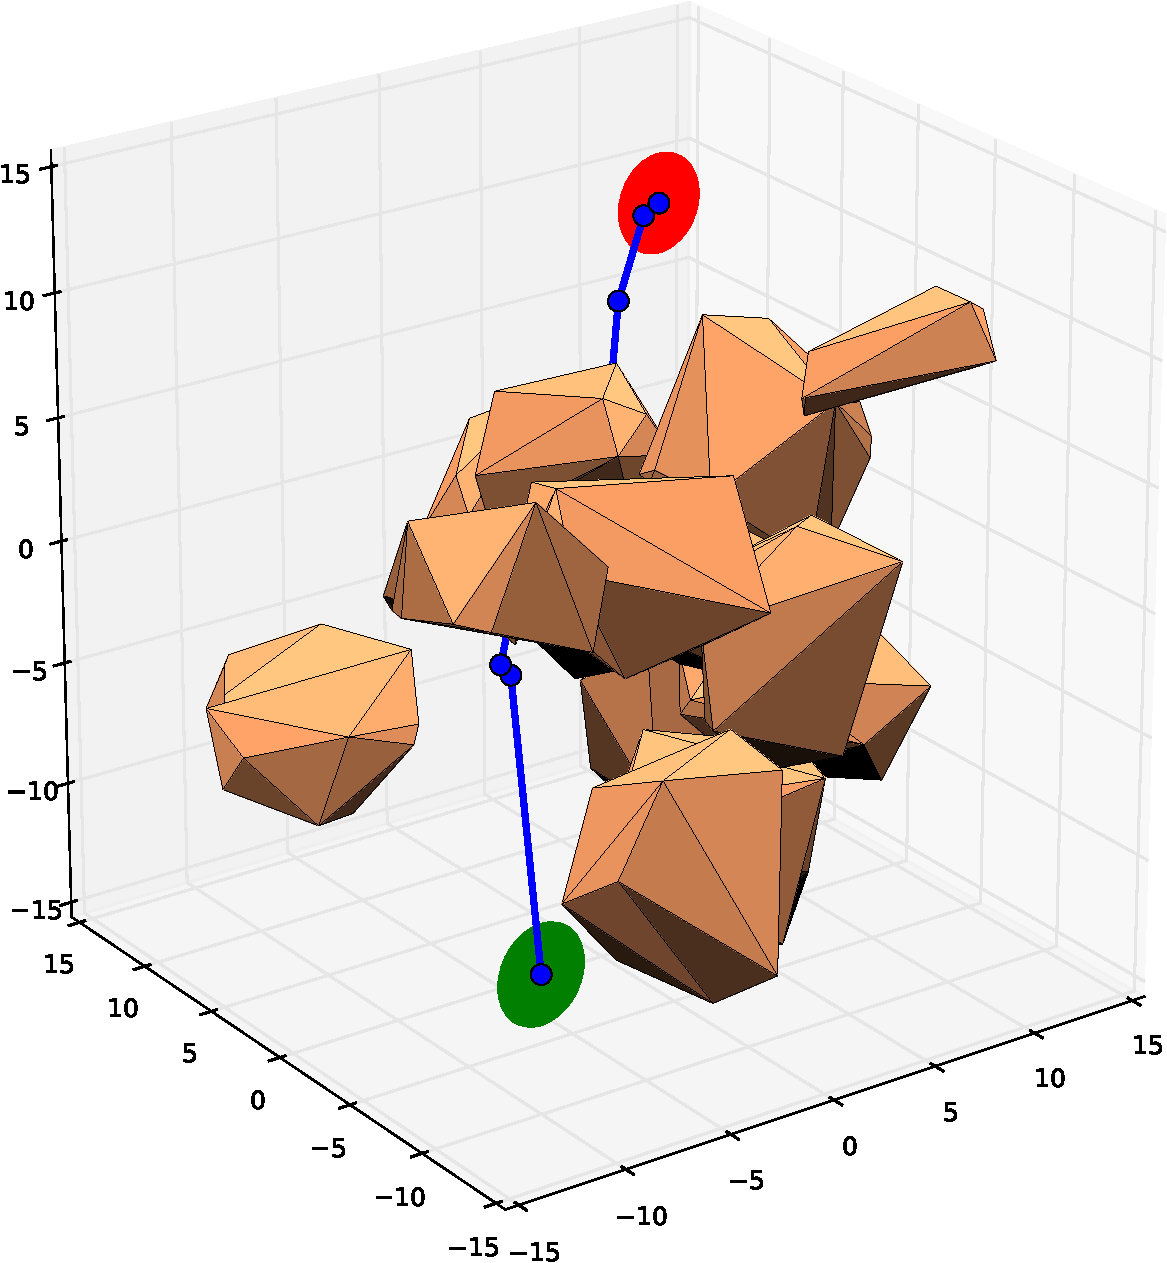
\includegraphics[width=\textwidth]{3d_example_2.pdf}
        \caption{b}
    \end{subfigure}
    \begin{subfigure}[t]{0.32\textwidth}
        \centering
        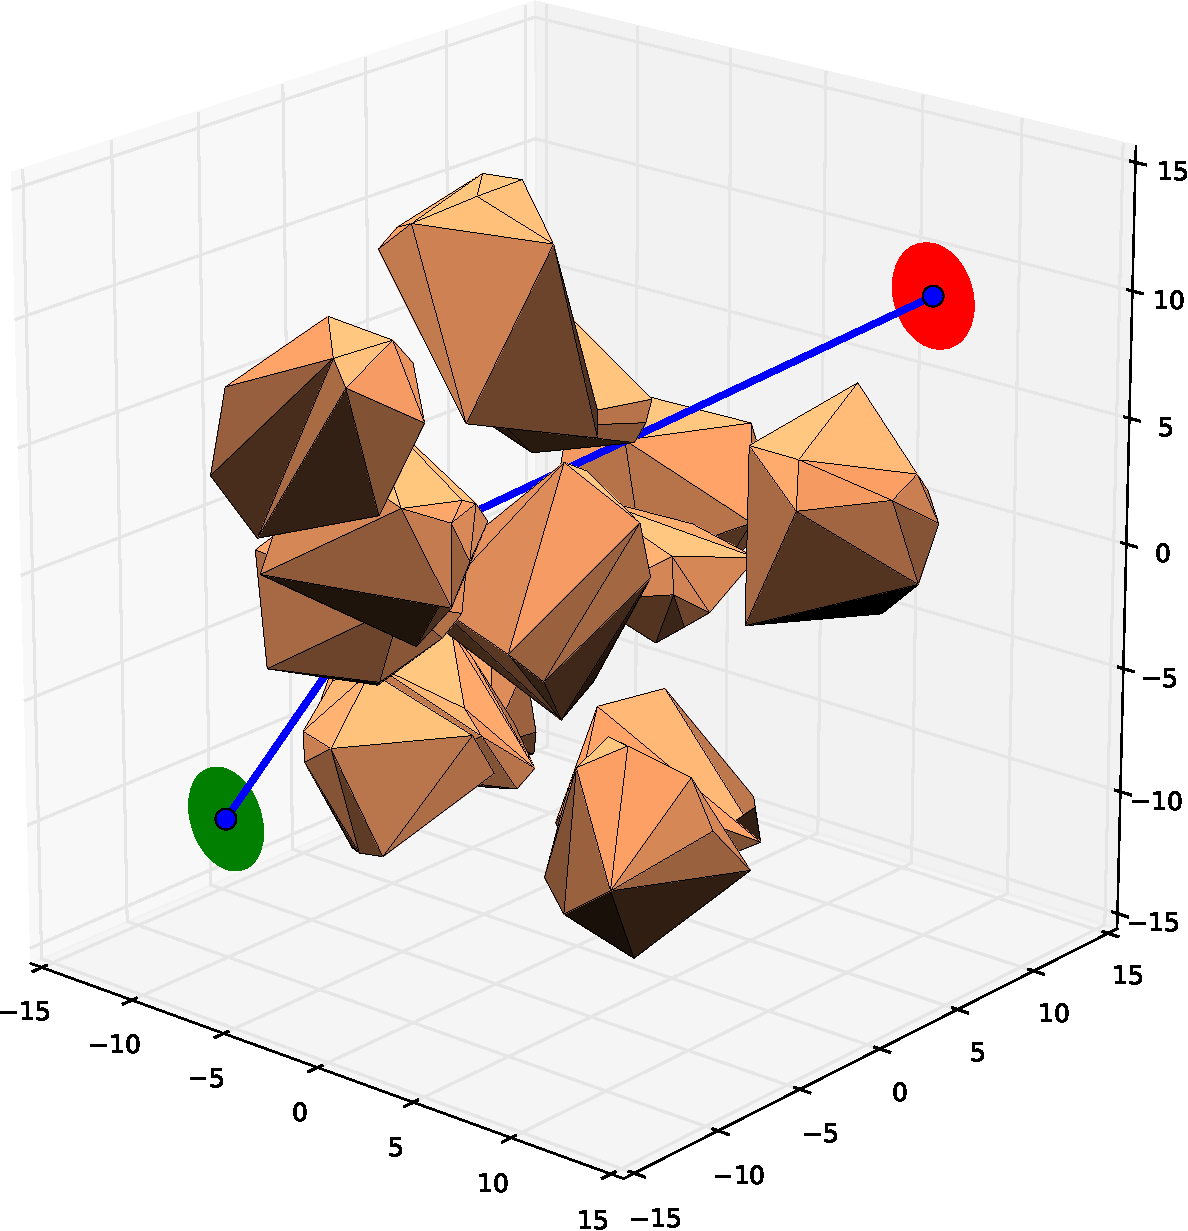
\includegraphics[width=\textwidth]{3d_example_3.pdf}
        \caption{c}
    \end{subfigure}
    \caption{3d examples}
    \label{fig:3d_examples}
\end{figure}

You can see examples of our code running in Fig ~\ref{fig:3d_examples}. The results are listed in Figure WHAT. They show that 

\begin{algorithm}[ht] 
    \caption{$\Function{PRM}^*$~\cite{karaman2011sampling}}
    \label{alg:PRMstar}
    \begin{algorithmic}[1]
        \setcounter{ALC@line}{0}
        \vspace*{1mm}

        \STATE $V \leftarrow \{x_{\Var{init}}\} \cup \{\Var{SampleFree}_i\}_{i=1,\ldots,n}$
        \STATE $E \leftarrow \emptyset$
        \FORALL{$v \in V$}
            \STATE $U \leftarrow \Function{Near}(G = (V, E), v,
            \gamma \cdot \Function{PRM}(\log(n) / n) ^ {1 / d})
            \backslash \{v\}$
            \FORALL{$u \in U$}
                \IF{$\Function{CollisionFree}(v, u)$}
                    \STATE $E \leftarrow E \cup \{(v, u), (u, v)\}$
                \ENDIF
            \ENDFOR
        \ENDFOR
        \RETURN $G = (V, E)$

    \end{algorithmic}
\end{algorithm}

\begin{algorithm}[ht] 
    \caption{$\Function{RRT}^*$~\cite{karaman2011sampling}}
    \label{alg:RRTstar}
    \begin{algorithmic}[1]
        \setcounter{ALC@line}{0}
        \vspace*{1mm}

        \STATE $V \leftarrow \{x_{\Var{init}}\}$
        \STATE $E \leftarrow \emptyset$
        \FOR{$i = 1 \ \TO \ n$}
            \STATE $\xr \leftarrow \Var{SampleFree}_i$
            \STATE $\xnearest \leftarrow \Function{Nearest}(G = (V, E), \xr)$
            \STATE $\xnew \leftarrow \Function{Steer}(\xnearest, \xr)$
            \IF{$\Function{ObstacleFree}(\xnearest, \xnew)$}
                \STATE $\xnear \leftarrow \Function{Near}(G = (V, E), \xnew,
                \min \{\gamma \cdot \Function{RRT}(\log(|V|) / |V|)^{1 / d}, \eta\})$
                \STATE $V \leftarrow V \cup \{\xnew\}$
                \STATE $\xmin \leftarrow \xnearest$
                \STATE $\cmin \leftarrow \Function{Cost}(\xnear) +
                c(\Function{Line}(\xnearest, \xnew))$
                \FORALL{$\xnear \in X_{\Var{near}}$}
                    \STATE $C \leftarrow \cost(\xnear) + \linef{\xnear, \xnew}$
                    \IF{$\Function{CollisionFree}(\xnear, \xnew) \wedge C < \cmin$}
                        \STATE $\xmin \leftarrow \xnear$
                        \STATE $\cmin \leftarrow C$
                    \ENDIF
                    \STATE $E \leftarrow E \cup \{(\xmin, \xnew)\}$
                \ENDFOR
                \FORALL{$\xnear \in X_{\Var{near}}$}
                    \STATE $C \leftarrow \cost(\xnew) + \linef{\xnew, \xnear}$
                    \IF{$\Function{CollisionFree}(\xnew, \xnear) \wedge C < \cost(\xnear)$}
                        \STATE $\xparent \leftarrow \Function{Parent}(\xnear)$
                        \STATE $E \leftarrow (E \backslash \{(\xparent, \xnear)\}) \cup \{(\xnew, \xnear)\}$
                    \ENDIF
                \ENDFOR
            \ENDIF
        \ENDFOR
        \RETURN $G = (V, E)$

    \end{algorithmic}
\end{algorithm}

\begin{algorithm}[ht] 
    \caption{$\Function{Dimensionality Reduction}$}
    \label{alg:DR}
    \begin{algorithmic}[1]
        \setcounter{ALC@line}{0}
        \vspace*{1mm}

        \STATE $Specify dimension, dimensionality reduction technique, and obstacle information$
        \STATE $Generate obstacles based off of obstacle information$
        \STATE $Fit dimensionality reduction transform to the space$
        \STATE $Transform the space$
        \STATE $Run PRM* over the space$
        \STATE $Inverse transform the path back to the original dimension$
        \STATE $Check for collisions$
    \end{algorithmic}
\end{algorithm}


\bibliographystyle{plain}
\bibliography{bib}

\end{document}
